\documentclass[11pt]{report}
\usepackage[margin=2cm]{geometry}
\usepackage{graphicx}
\usepackage{float}
\usepackage{times}
\usepackage{url}
\usepackage[dvipsnames]{xcolor}

\newcommand{\Gap}{\texorpdfstring{\hfill}{}}
\newcommand{\Rec}{\texorpdfstring{{\small\emph{\color{blue}{\fbox{High Leverage}}}}}{}}
\newcommand{\HighRisk}{\texorpdfstring{{\small\emph{\color{orange}{\fbox{Uncertain Impact}}}}}{}}
\newcommand{\Longterm}{\texorpdfstring{{\small\emph{\color{OliveGreen}{\fbox{Long-term}}}}}{}}

\begin{document}
\section{Climate Prediction\texorpdfstring{\hfill\textit{by Kelly Kochanski}}{}}
\label{sec: climate prediction}


The first global warming prediction was made in 1896, when Arrhenius estimated that burning fossil fuels could eventually release enough CO$_2$ to warm the Earth by $5^\circ$C.
The fundamental physics underlying those calculations has not changed, but our predictions have become far more detailed and precise. The predominant predictive tools are climate models, known as \emph{General Circulation Models (GCMs)} or \emph{Earth System Models (ESMs)}\footnote{Learn about climate modeling from \url{climate.be/textbook} \cite{Goosse} or Climate Literacy, \url{youtu.be/XGi2a0tNjOo}}. These models inform local and national government decisions (see IPCC reports \cite{ipcc2014summary,IPCC2014,ipcc_global_2018}), help people calculate their climate risks (see \textsection\ref{sec:tools-individuals} and \textsection\ref{sec:societal-impacts}) and allow us to estimate the potential impacts of solar geoengineering (see \textsection\ref{sec:geoengineering}).

Recent trends have created opportunities for ML to advance the state-of-the-art in climate prediction (Fig.~\ref{fig:climateModels}). First, new and cheaper satellites are creating petabytes of climate observation data\footnote{e.g.~NASA's Earth Science Data Systems program, \url{earthdata.nasa.gov}, and ESA's Earth Online, \url{earth.esa.int}}. Second, massive climate modeling projects are generating petabytes of simulated climate data\footnote{e.g.~the Coupled Model Intercomparison Project, \url{cmip.llnl.gov} \cite{Taylor2012, Eyring2016} and Community Earth System Model Large Ensemble \cite{Kay2015}}. Third, climate forecasts are computationally expensive \cite{Carman2017} (the simulations in \cite{Kay2015} took three weeks to run on NCAR supercomputers), while ML methods are becoming increasingly fast to train and run, especially on next-generation computing hardware. As a result, climate scientists have recently begun to explore ML techniques, and are starting to team up with computer scientists to build new and exciting applications.

\begin{figure}[bhpt]
    \centering
    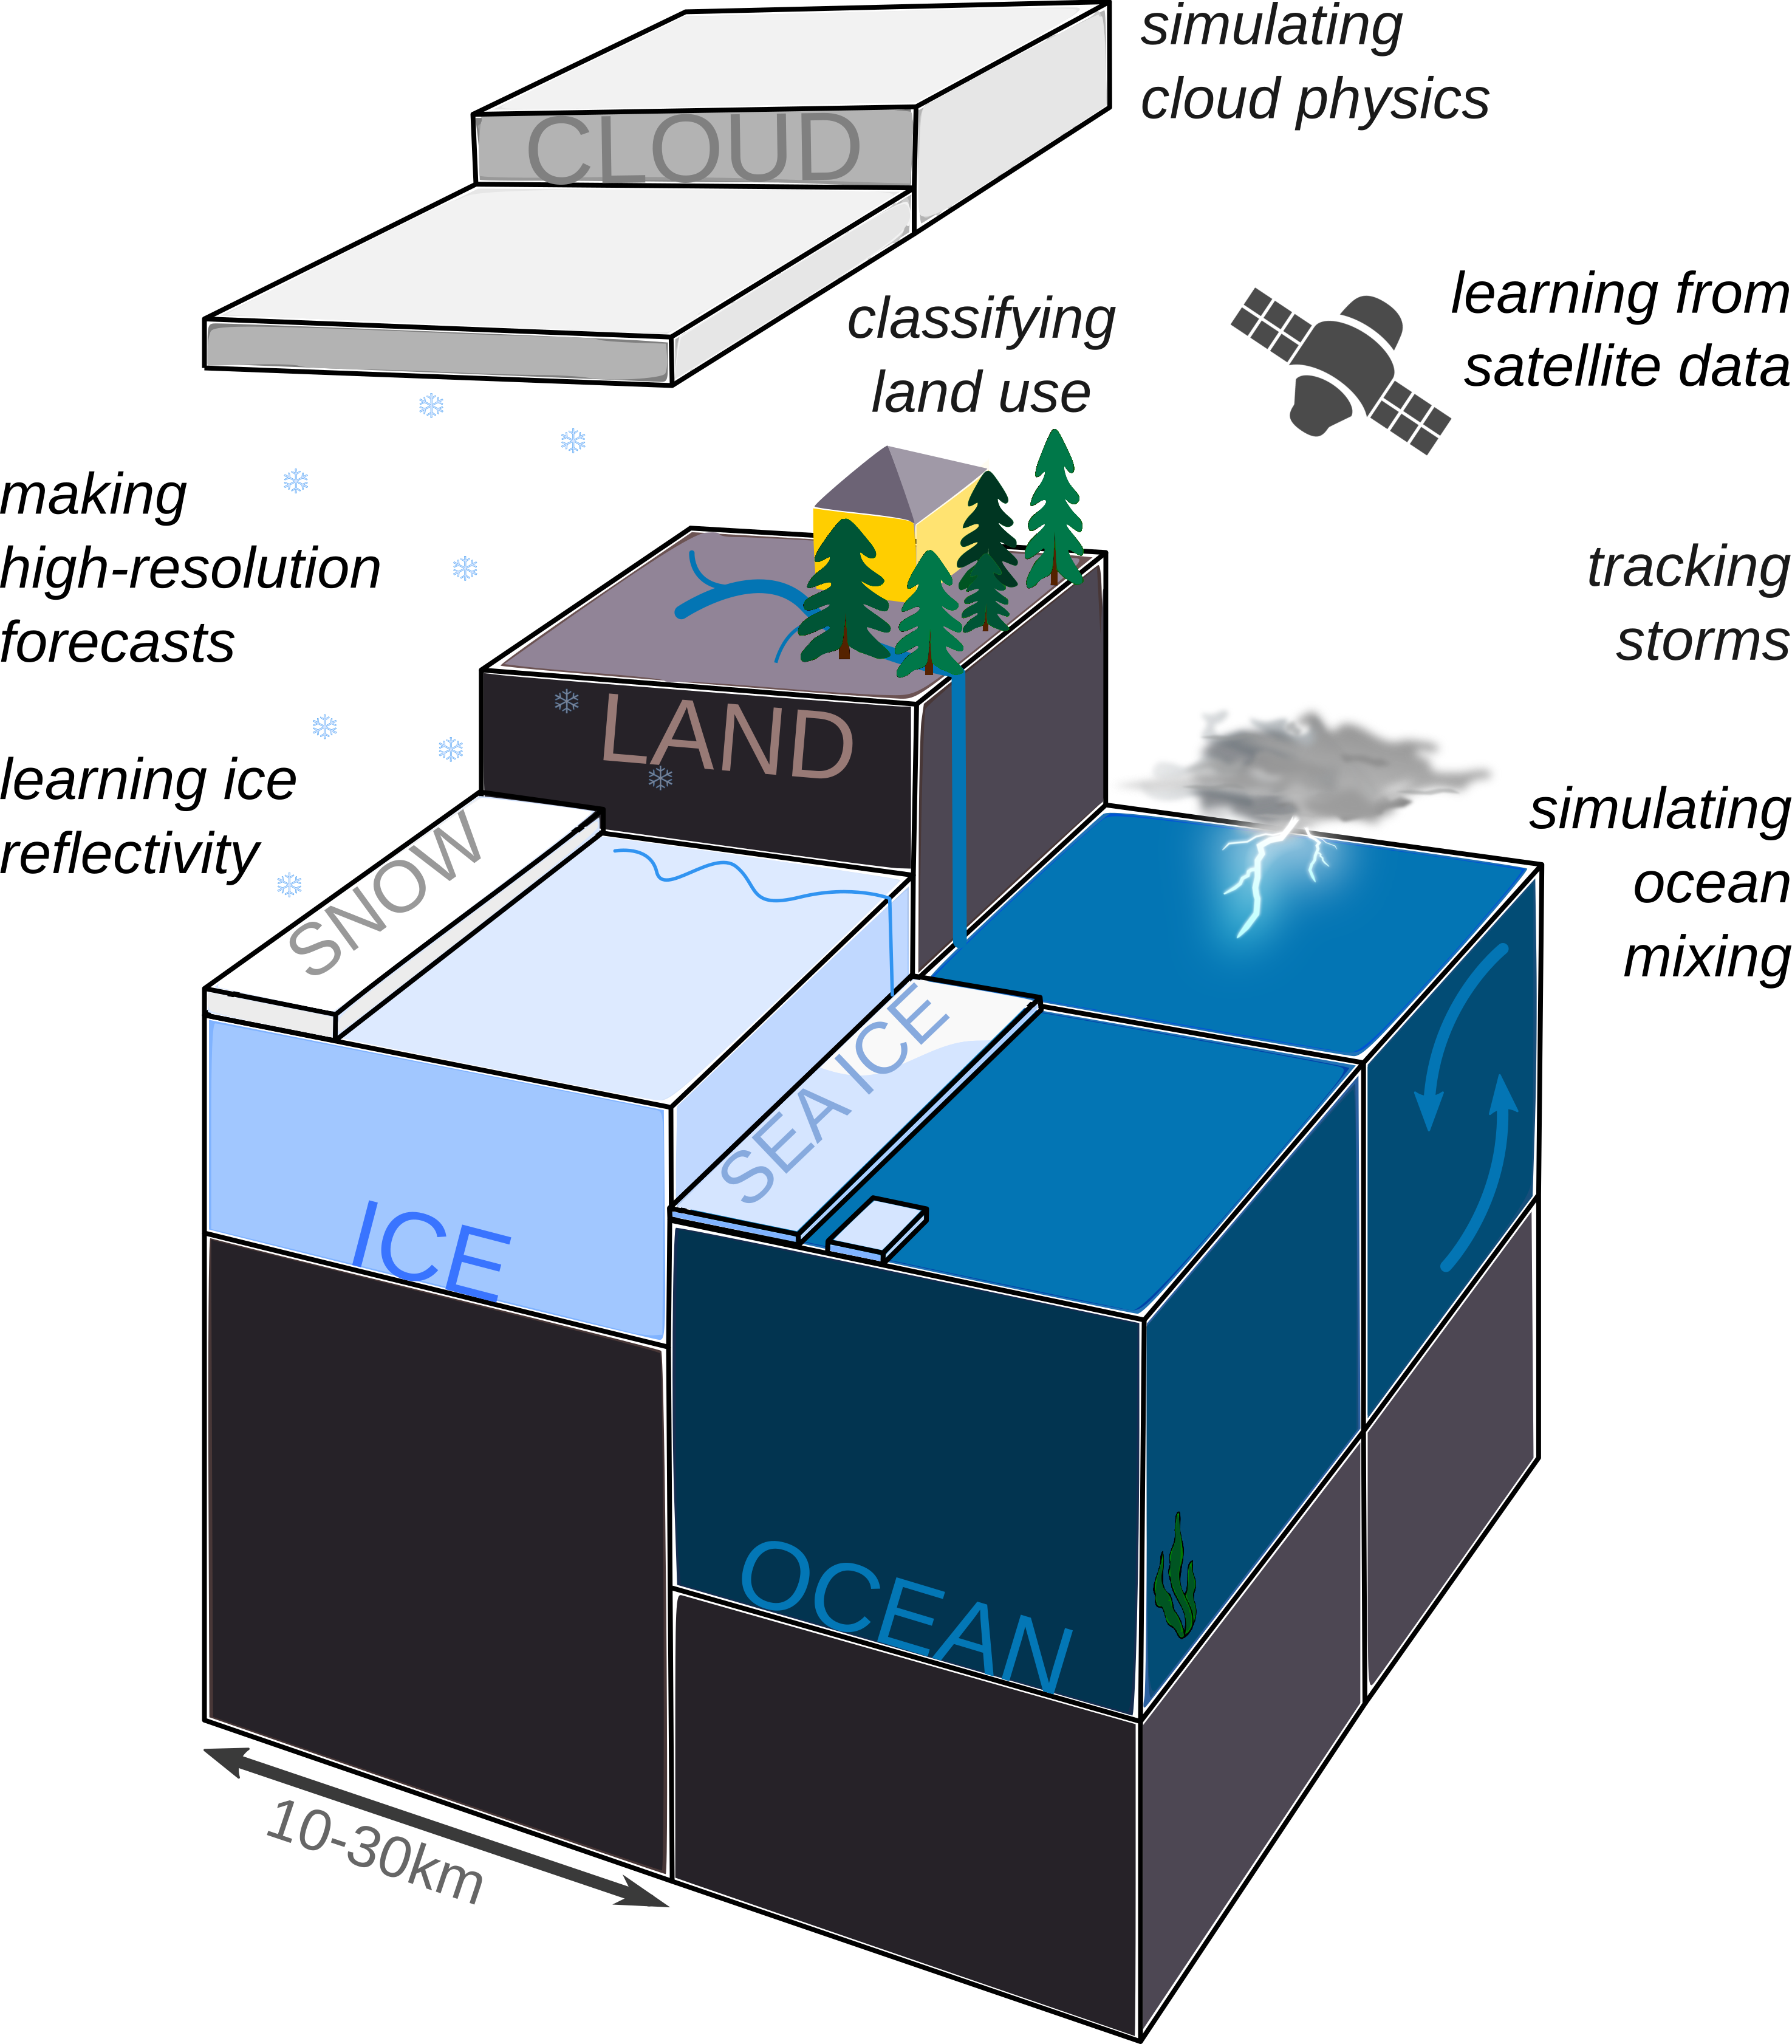
\includegraphics[width=8.7cm]{figures/climate_prediction.png}
    \caption{Schematic of a climate model, with selected strategies to improve climate change predictions using machine learning.}
    \label{fig:climateModels}
\end{figure}

\subsection{Uniting data, ML, and climate science}
\label{sec:climate-models-params}
Climate models represent our understanding of Earth and climate physics. We can learn about the Earth by collecting data. To turn that data into useful predictions, we need to condense it into coherent, computationally tractable models.
ML models are likely to be more accurate or less expensive than other models where:
(1) there is plentiful data, but it is hard to model systems with traditional statistics, or
(2) there are good models, but they are too computationally expensive to use in production.

\subsubsection{Data for climate models}
When data are plentiful, 
climate scientists build data-driven models. In these areas, ML techniques may solve many problems that were previously challenging.
These include black box problems, for instance sensor calibration \cite{Lary2009}, and classification of observational data, for instance classifying crop cover or identifying pollutant sources in satellite imagery \cite{Lary2015,Kussul2017}.
More applications like these are likely to appear as satellite databases grow. 
The authors of \cite{Monteleoni2013chapter} describe many opportunities for data scientists to assimilate data from diverse field and remote sensing sources, many of which have since been explored by climate informatics researchers.

Numerous authors, such as \cite{Gil2019}, have identified geoscience problems that would be aided by the development of benchmark datasets. Efforts to develop such datasets include
EnviroNet \cite{Mukkavilli2019}, the IS-GEO benchmark datasets \cite{Ebert2017}, and ExtremeWeather \cite{Racah2017}. 
We expect the collection of curated geoscience datasets to continue to grow;
this process might even be accelerated by ML optimizations in data collection systems \cite{Gil2019}.
We strongly encourage modellers to dive into the data in collaboration with domain experts.
We also recommend that modellers who seek to learn directly from data see \cite{Hourdin2017} for specific advice on fitting and over-fitting climate data.


\subsubsection{Accelerating climate models}
Many climate prediction problems are irremediably data-limited. No matter how many weather stations we construct, how many field campaigns we run, or how many satellites we deploy, the Earth will generate at most one year of new climate data per year. Existing climate models deal with this limitation by relying heavily on physical laws, such as thermodynamics.
These models are structured in terms of coupled partial differential equations that represent physical processes like cloud formation, ice sheet flow, and permafrost melt.
ML models provide new techniques for solving such systems efficiently.

\paragraph*{Clouds and aerosols}\Gap\textbf{\Rec}\mbox{}\\
Recent work has shown how deep neural networks could be combined with existing thermodynamics knowledge to fix the largest source of uncertainty in current climate models: clouds. Bright clouds block sunlight and cool the Earth; dark clouds catch outgoing heat and keep the Earth warm \cite{IPCC2014, Sherwood2014}. These effects are controlled by small-scale processes such as cloud convection and atmospheric aerosols (see uses of aerosols for cloud seeding and solar geoengineering in \textsection\ref{sec:geoengineering}). Physical models of these processes are far too computationally expensive to include in global climate models --- but ML models are not. Gentine et al.~trained a deep neural network to emulate the behavior of a high-resolution cloud simulation, and found that the network gave similar results for a fraction of the cost \cite{Gentine2018} and was stable in a simplified global model \cite{Rasp2018}. Existing scientific model structures do not always offer great trade-offs between cost and accuracy. Neural networks trained on those scientific models produce similar predictions, but offer an entirely new set of compromises between training cost, production cost, and accuracy. Replacing select climate model components with neural network approximators may thus improve both the cost and the accuracy of global climate models. Additional work is needed to identify more climate model components that could be replaced by neural networks (we highlight other impactful components below), to optimize those models, and to automate their training workflows (see examples in \cite{Reichstein2019}).

\paragraph{Ice sheets and sea level rise}\Gap\textbf{\Rec}\mbox{}\\
The next most important targets for climate model improvements are ice sheet dynamics and sea level rise. The Arctic and Antarctic are warming faster than anywhere else on Earth, and their climates control the future of global sea level rise and many vulnerable ecosystems \cite{ipcc2014summary, ipcc_global_2018}. Unfortunately, these regions are dark and cold, and until recently they were difficult to observe. In the past few years, however, new satellite campaigns have illuminated them with hundreds of terabytes of data\footnote{See e.g.~\url{icebridge.gsfc.nasa.gov} and \url{pgc.umn.edu/data/arcticdem}.}. These data could make it possible to use ML to solve some of the field's biggest outstanding questions. In particular, models of mass loss from the Antarctic ice-sheet are highly uncertain \cite{Kopp2017} and models of the extent of Antarctic sea ice do not match reality well \cite{Gagne2015}. The most uncertain parts of these models, and thus the best targets for improvement, are snow reflectivity, sea ice reflectivity, ocean heat mixing and ice sheet grounding line migration rates \cite{Hourdin2017,Kopp2017,Hanna2013}. Computer scientists who wish to work in this area could build models that learn snow and sea ice properties from satellite data, or use new video prediction techniques to predict short-term changes in the sea ice extent.

\subsubsection{Working with climate models}
ML could also be used to identify and leverage relationships between climate variables. Pattern recognition and feature extraction techniques could allow us to identify more useful connections in the climate system, and regression models could allow us to quantify non-linear relationships between connected variables. For example, Nowack et al.~demonstrated that ozone concentrations could be computed as a function of temperature, rather than physical transport laws, which led to considerable computational savings \cite{Nowack2018}.

The best climate predictions are synthesized from ensembles of 20+ climate models \cite{Tebaldi2007}. Making good ensemble predictions is an excellent ML problem. Monteleoni et al.~proposed that online ML algorithms could create better predictions of one or more target variables in a multi-model ensemble of climate models \cite{Monteleoni2011}; this idea has been refined in \cite{Mcquade2012,Strobach2015}. More recently, Anderson and Lucas used random forests to make high-resolution predictions from a mix of high- and low-resolution models, which could reduce the costs of building multi-model ensembles \cite{Anderson2018}. 
 

In the further future, the Climate Modeling Alliance has proposed to build an entirely new climate model that learns continuously from data and from high-resolution simulations \cite{Schneider2017}. The proposed model would be written in Julia, in contrast to existing models which are mostly written in C++ and Fortran. At the cost of a daunting translation workload, they aim to build a model that is more accessible to new developers and more compatible with ML libraries.

\subsection{Forecasting extreme events}
\label{sec:models-extreme-events}
For most people, extreme event prediction means the local weather forecast and a few days' warning to stockpile food, go home, and lock the shutters.
Weather forecasts are shorter-term than climate forecasts, but they produce abundant data. Weather models are optimized to track the rapid, chaotic changes of the atmosphere; since these changes are fast, tomorrow's weather forecast is made and tested every day. Climate models, in contrast, are chaotic on short time scales, but their long-term trends are driven by slow, predictable changes of ocean, land, and ice (see \cite{Shukla1998})\footnote{This is one of several reasons why climate models produce accurate long-term predictions in spite of atmospheric chaos.}. As a result, climate model output can only be tested against long-term observations (at the scale of years to decades).  Intermediate time scales, of weeks to months, are exceptionally difficult to predict, although Cohen et al.~\cite{Cohen2018} argue that machine learning could bridge that gap by making good predictions on four to six week timescales \cite{Hwang2019}. Thus far, however, weather modelers have had hundreds of times more test data than climate modelers, and began to adopt ML techniques earlier. Numerous ML weather models are already running in production. For example, Gagne et al.~recently used an ensemble of random forests to improve hail predictions within a major weather model \cite{Gagne2017}. 

A full review of the applications of ML for extreme weather forecasting is beyond the scope of this article. Fortunately, that review has already been written: see \cite{McGovern2017using}.
The authors describe ML systems that correct bias, recognize patterns, and predict storms. Moving forward, they envision human experts working alongside automated forecasts.

\subsubsection{Storm tracking}
Climate models cannot predict the specific dates of future events, but they can predict changes in long-term trends like drought frequency and storm intensity. Information about these trends helps individuals, corporations and towns make informed decisions about infrastructure, asset valuation and disaster response plans (see also \S\ref{subsub:crisis}). Identifying extreme events in climate model output, however, is a classification problem with a twist: all of the available data sets are strongly skewed because extreme events are, by definition, rare. ML has been used successfully to classify some extreme weather events.
Researchers have used deep learning to classify \cite{Liu2016}, detect \cite{Racah2017} and segment \cite{Kurth2018} cyclones and atmospheric rivers, as well as tornadoes \cite{Lakshmanan2010}, in historical climate datasets.
Tools for more event types would be useful, as would online tools that work within climate models, labelled datasets for predicting future events, and statistical tools that quantify the uncertainty in new extreme event forecasts.

\subsubsection{Local forecasts \Gap \Rec}
Forecasts are most actionable if they are specific and local. ML is widely used to make local forecasts from coarse 10--100 km climate or weather model predictions; various authors have attempted this using support vector machines, autoencoders, Bayesian deep learning, and super-resolution convolutional neural networks (e.g.~\cite{Li2019}). Several groups are now working to translate high-resolution climate forecasts into risk scenarios. For example, ML can predict localized flooding patterns from past data \cite{perignon2018patterns}, which could inform individuals buying insurance or homes. Since ML methods like neural networks are effective at predicting local flooding during extreme weather events \cite{sit2019decentralized}, these could be used to update local flood risk estimates to benefit individuals. The start-up Jupiter Intelligence
is working to make climate predictions more actionable by translating climate forecasts into localised flood and temperature risk scores.

\subsection{Discussion}
\label{sec: climate models - ml+science}
 ML may change the way that scientific modeling is done. The examples above have shown that many components of large climate models can be replaced with ML models at lower computational costs. 
 From an ML standpoint, learning from an existing model has many advantages: modelers can generate new training and test data on-demand, and the new ML model inherits some community trust from the old one. This is an area of active ML research.
 Recent papers have explored data-efficient techniques for learning dynamical systems \cite{Raissi2018}, including physics-informed neural networks \cite{Raissi2017} and neural ordinary differential equations \cite{chen2018neural}. In the further future, researchers are developing ML approaches for a wide range of scientific modeling challenges, including crash prediction \cite{Lucas2013}, adaptive numerical meshing \cite{Jiang2016}, uncertainty quantification \cite{Ling2015, Lakshminarayanan2017} and performance optimization \cite{Thiagarajan2018}. If these strategies are effective, they may solve some of the largest structural challenges facing current climate models.
 
New ML models for climate will be most successful if they are closely integrated into existing scientific models. This has been emphasized, again and again, by authors who have laid future paths for artificial intelligence within climate science \cite{Lary2018,Gil2019,Rasp2018,McGovern2017using,Reichstein2019,Schneider2017}. New models need to leverage existing knowledge to make good predictions with limited data. In ten years, we will have more satellite data, more interpretable ML techniques, hopefully more trust from the scientific community, and possibly a new climate model written in Julia. For now, however, ML models must be creatively designed to work within existing climate models. The best of these models are likely to be built by close-knit teams including both climate and computational scientists.


\end{document}
